
%%%%%%%%%%%%%%%%%%%%%%%%%%%%%%%%%%%%%%%%%%%%%%%%%%%%%%%%%%%%%%%%%%%%%%%%%%%%%%
%                                                                            %
%  ************************** AVISO IMPORTANTE **************************    %
%                                                                            %
% Éste es un documento de ayuda para los autores que deseen enviar           %
% trabajos para su consideración en el Boletin de la Asociación Argentina    %
% de Astronomía.                                                             %
%                                                                            %
% Los comentarios en este archivo contienen instrucciones sobre el formato   %
% obligatorio del mismo que complementan los instructivos web y PDF.         %
% Por favor léalos.                                                          %
%                                                                            %
% No deben borrarse los comentarios en este archivo. En caso contrario,      %
% el sistema de recepción de manuscritos no permitirá el envío de su         %
% contribución. No se permite el uso de \newcommand ni definiciones          %
% particulares de cada autor.                                                %
%                                                                            %
%%%%%%%%%%%%%%%%%%%%%%%%%%%%%%%%%%%%%%%%%%%%%%%%%%%%%%%%%%%%%%%%%%%%%%%%%%%%%%

%%%%%%%%%%%%%%%%%%%%%%%%%%%%%%%%%%%%%%%%%%%%%%%%%%%%%%%%%%%%%%%%%%%%%%%%%%%%%%
%                                                                            %
%  ************************** IMPORTANT NOTICE **************************    %
%                                                                            %
%  This is a help file for authors who are preparing manuscripts to be       %
%  considered for publication in the Boletin de la Asociación Argentina      %
%  de Astronomía.                                                            %
%                                                                            %
%  The comments in this file give instructions about the manuscripts'        %
%  mandatory format that complement the instructions distributed as a PDF    %
%  and findable in the BAAA web. Please read them.                           %
%                                                                            %
%  The comments in this file must not be deleted. Otherwise, your            %
%  contribution will be rejected by the manuscript reception system.         %
%  The use of \newcommand and author definitions are forbidden.              %
%                                                                            %
%%%%%%%%%%%%%%%%%%%%%%%%%%%%%%%%%%%%%%%%%%%%%%%%%%%%%%%%%%%%%%%%%%%%%%%%%%%%%%

\documentclass[baaa]{baaa}

\usepackage[pdftex]{hyperref}
\usepackage{subfigure}
\usepackage{natbib}
\usepackage{helvet,soul}
\usepackage[font=small]{caption}
\usepackage{float}
\usepackage{graphicx}


% Defino clases de secciones en ESPAÑOL
\def\chaptername{Cap\'\i tulo}
\def\abstractname{Resumen}
\def\contentsname{Contenidos}
\def\bibname{Bibliograf\'\i a}
\def\appendixname{Ap\'endice}
\def\tablename{\textbf{Tabla}}
\def\figurename{\textbf{Figura}}
%\usepackage[dvips]{graphics,color,epsfig}
%\usepackage{pst-all}
%\usepackage{pstricks}
%\topmargin=-2cm  

% Defino formatos
\def\titulo#1{\frametitle{{\ \hfill {\bf #1}}}}
\def\figu#1{\shadowbox{#1}}

\def\Eeuv{E_{\rm{EUV}}}
\def\Ewl{E_{\rm{WL}}}
\def\AvgNE2{\left<N_e^2\right>}
\def\AvgNe{\left<N_e\right>}
\def\SigmaNe{\sigma_{Ne}}
\def\VarNe{\rm{Var}N_e}
\def\AvgTe{\left<T_e\right>}
\def\SigmaTe{\sigma_{Te}}


%EStilo
%\input{epsf.sty}

%Paquetes a utilizar

%\usepackage{amssymb} % Math
%\usepackage{graphicx}
%\usepackage{float}
%%\usepackage{wrapfig}
%%\usepackage{deluxetable}

\pagenumbering{arabic}
%\usepackage[dvips]{graphics,color}
%\usepackage{natbib}
%\usepackage{amssymb} % Math
%\usepackage{amsmath} % Math
%%\usepackage{dsfont} % Math
%\usepackage{float}
%\usepackage{graphicx}
%%\usepackage{wrapfig}
%\usepackage{pst-all}
%%\usepackage{multirow} % Multi filas

%Separacion silabica:
%%\usepackage[T1]{babel} % silabas y hyphenation
%\hyphenation{e-vi-den-cia}
%\hyphenation{an-te-rio-res}

% Control de Márgenes

%-------------------- Comandos de los autores ----------------------------

% Nombres de Journals
%\newcommand{\araa}{Annu. Rev. Astron. Astrophys.}
%\newcommand{\solphys}{Solar Phys.}
%\newcommand{\aapr}{Astron. Astrophys. Rev.}
%\newcommand{\aaps}{Astron. Astrophys. Sup. Ser.}
%\newcommand{\jastp}{Jour. Atmos. Solar-Terrestrial Phys.}
%\newcommand{\pasj}{Pub. Astron. Soc. Japan}
%\newcommand{\etal}{et al.\ }
%\newcommand{\ha}{H$\alpha$ }
%\newcommand{\aap}{Astron. \& Astrophys.}
%\newcommand{\apjs}{Astrophys J. Sup.}
%\newcommand{\jgr}{Journal of Geophys. Res.}
%\newcommand{\grl}{Geophys. Res. Let.}
%\newcommand{\pre}{Physical Rev. E}
%\newcommand{\adv}{Adv. in Space Res.}
%\newcommand{\SpaceS}{Space Science Reviews}
%\newcommand{\planss}{Planet. Space Sci.}
%\newcommand{\nat}{Nature}
%\newcommand{\apj}{The Astrophysical Journal}
%\newcommand{\apjS}{The Astrophysical Journal Supplement}
%\newcommand{\apjl}{The Astrophysical Journal Letters}
%\newcommand{\mnras}{MNRAS}
%\newcommand{\pasp}{Publications of the Astronomical Society of the Pacific}
%\newcommand{\apss}{Astrophys. Space Sci.}

% Formato
\def\salto{\vskip 0.3cm}
\def\mediosalto{\vskip 0.15cm}

% Math:
\def\deg{$^\circ$}
\def\rsun{R$_{\odot}$}
\def\bB{\mathbf{B}}
\def\bE{\mathbf{E}}
\def\dpar#1#2{\frac{\partial#1}{\partial#2}}
%color:
\def\red#1{{\textcolor{red}{#1}}}
\def\azul#1{{\textcolor{blue}{#1}}}

\def\Figura#1{Figura \ref{#1}}
\def\Figuras#1#2{Figuras \ref{#1} a \ref{#2}}
\def\Figurasy#1#2{Figuras \ref{#1} y \ref{#2}}
\def\Tabla#1{Tabla \ref{#1}}
\def\Eq#1{Ecuaci\'on (\ref{#1})}
\def\Eqs#1#2{Ecuaciones (\ref{#1})-(\ref{#2})}
\def\Eqn#1{Ecuaci\'on (\ref{#1})}
\def\eqsy#1#2{Ecuaciones (\ref{#1}) y (\ref{#2})}

\def\exp{{\rm exp}}
\def\ln{{\rm ln}}
\def\sin#1{{\rm sen}(#1)}
\def\cos#1{{\rm cos}(#1)}
\def\sec{{\rm sec}}
\def\erg{{\rm erg}}
\def\cm{{\rm cm}}
\def\km{{\rm km}}
\def\sr{{\rm sr}}
\def\Hz{{\rm Hz}}
\def\GHz{{\rm GHz}}
\def\kev{{\rm kev}}
\def\sfu{{\rm SFU}}
\def\K{{\rm K}}
\def\MK{{\rm MK}}
\def\AU{{\rm UA}}
\def\UA{{\rm UA}}
\def\Log10{{\rm log_{10}}}
\def\G{{\rm G}}
\def\gsun{g_{\odot}}
\def\Rsun{R_{\odot}}
\def\Msun{ M_{\odot}}
\def\Ne{N_\mathrm{e}}
\def\NH{N_\mathrm{H}}
\def\NHe{N_\mathrm{He}}
\def\me{m_\mathrm{e}}
\def\mH{m_\mathrm{H}}
\def\mHe{m_\mathrm{He}}
\def\Tm{T_m}
\def\Tfit{T_{\rm fit}}
\def\Tefit{T_{e,{\rm fit}}}
\def\Te{T_{\rm e}}
\def\TH{T_{\rm H}}
\def\THe{T_{\rm He}}
\def\l{\lambda_{{\rm N}}}
\def\WT{W_{T}}
\def\aTm{\left<\Tm\right>}
\def\dT{\Delta T}
\def\emisin{\zeta_k^{\rm (syn)}}
\def\emitom{\zeta_k^{\rm(tom)}}

\def\fa{f_{\alpha} ({\bf x},{\bf w},t)}
\def\ffa{f_\alpha}
\def\xt{({\bf x},t)}
\def\vt{({\bf v},t)}
\def\xw{({\bf x},{\bf w})}
\def\xwt{({\bf x},{\bf w},t)}
\def\fa{f_\alpha}
\def\ww{{\bf w}}
\def\xx{{\bf x}}
\def\uu{{\bf u}}
\def\kk{{\bf k}}
\def\V{{\bf V}}
\def\ga{{\bf \Gamma}}

\def\lD{\lambda_D}
\def\ve{v_{Te}}
\def\we{\omega_e}
%\def\me{m_e}

\def\dgdv{ \frac{\partial g}{\partial v} }

\def\dndt{ \frac{\partial n}{\partial t} }
\def\drhodt{ \frac{\partial \rho}{\partial t} }

\def\dfdt{ {{\partial f} \over {\partial t}} }
\def\dfdx{ {{\partial f} \over {\partial \xx}} }
\def\dfdw{ {{\partial f} \over {\partial \ww}} }

\def\ddv{ {{\partial} \over {\partial v}} }
\def\ddt{ {{\partial} \over {\partial t}} }
\def\ddx{ {{\partial} \over {\partial \xx}} }
\def\ddw{ {{\partial} \over {\partial \ww}} }

\def\ep{\epsilon}
\def\al{\alpha}
\def\om{\omega}
\def\EF{{\bf E}}
\def\BF{{\bf B}}
\def\dl{\lambda_D}

\def\wp{\om_{pe}}
\def\P{\buildrel =\over P}

\def\intindef{\int_{0}^{\infty}}
%-----------Albert's-----------------
\def\rmax{$R_{\rm max}$}
\def\Nrad{N_r}
\def\Nlat{N_\theta}
\def\Nlon{N_\phi}
\def\bzeta{\boldsymbol{\zeta}}
\def\bI{{\boldsymbol{I}}}
\def\bW{{\bf W}}
\def\bp{{\boldsymbol{p}}}
\def\bR{{\bf R}}
\def\AFe{A_{\rm Fe}}
\def\br{{\bf r}}
\def\bl{{\boldsymbol{\lambda}}}
\def\Tab#1{Tabla \ref{#1}}
\def\Tmin{T_{\rm min}}
\def\Tmax{T_{\rm max}}
\def\intmm{\int_{\Tmin}^{\Tmax}}

%------------------------de albert

%---------- Author's commands---------------------------------

\def\bu{\textcolor{red}{\textbullet~}}
\def\tr{\bu}
\def\bbu{\textbullet~}
\def\btr{\textcolor{blue}{$\triangleright$~}}
\def\cmsq{cm$^2$}
\def\cmcu{cm$^3$}
\def\azul#1{\textcolor{blue}{#1}}
\def\rojo#1{\textcolor{red}{#1}}
\def\verde#1{\textcolor{green}{#1}}
\def\orange#1{\textcolor{orange}{#1}}
\colorlet{green}{green!60!gray}




\def\rsun{R$_{\rm SUN}$}
\def\bA{{\bf A}}
\def\ba{{\boldsymbol{a}}}
\def\bB{{\bf B}}
\def\bb{{\bf b}}
\def\bC{{\bf C}}
\newcommand{\dd}{\mathrm{d}}
\def\bD{{\bf D}}
\def\bd{{\bf d}}
\def\be{{\boldsymbol{e}}}
\def\bF{{\bf F}}
\def\bff{{\bf f}}
\def\bg{{\bf g}}
\def\bG{{\bf G}}
\def\bh{{\bf h}}
\def\bH{{\bf H}}
\def\bi{{\bf i}}
\def\bI{{\boldsymbol{I}}}
\def\bk{{\bf k}}
\def\bK{{\bf K}}
\def\bM{{\bf M}}
\def\bn{{\boldsymbol{n}}}
\def\bv{{\boldsymbol{v}}}
\def\boo{{\boldsymbol{o}}}
\def\bp{{\boldsymbol{p}}}
\def\bP{{\bf $P$}}
\def\bq{{\boldsymbol{q}}}
\def\bQ{{\bf Q}}
\def\br{{\boldsymbol{r}}}
\def\bR{{\bf R}}
\def\bs{{\bf s}}
\def\bS{{\bf S}}
\def\bn{{\bf n}}
\def\bt{{\bf t}}
\def\bT{{\bf T}}
\def\bU{{\bf U}}
\def\bW{{\bf W}}
\def\bx{{\bf x}}
\def\by{{\bf y}}
\def\bSigma{{\bf \Sigma}}
\def\bLambda{{\bf \Lambda}}
\def\blambda{{\bf \lambda}}
\def\bN{{\bf \mathcal{N}}}
\def\bchi{\boldsymbol{\chi}}
\def\bxi{\boldsymbol{\xi}}
\def\bzeta{\boldsymbol{ \zeta}}
\newcommand{\lbl}{\mbox{\boldmath $\hat{l}$}}
\newcommand{\lpl}{\mbox{\boldmath $\hat{p}$}}
\def\deg{$^\circ$}
\def\mdeg{^\circ}
\def\bbp{{\bf p}}

%\def\tr{\textcolor{blue}{$\blacktriangleright$~}}
\def\bu{\textcolor{blue}{\textbullet~}}
\def\tr{\bu}
\def\bbu{\textbullet~}

\def\cmsq{cm$^2$}
\def\cmcu{cm$^3$}

\def\azul#1{\textcolor{blue}{#1}}
\def\rojo#1{\textcolor{red}{#1}}
\def\verde#1{\textcolor{green}{#1}}
\def\orange#1{\textcolor{orange}{#1}}

\def\bL{{\bf L}}
\def\bE{{\bf E}}

% Author's commands:
\newcommand{\DT}{\Delta T}
\newcommand{\Tsyn}{T_{\rm Syn}}
\newcommand{\Texp}{T_{\rm exp}}
\newcommand{\seg}{{\rm seg}}


%Simbolos
\def\izquierda{\azul{$\bf\leftarrowtail$}}
\def\derecha{\azul{$\bf\rightarrowtail$}}

%Diego:
\def\mrsun{{\rm R_\odot}}
\def\avgTe{\left<T_e\right>}
\def\bfa#1{\textcolor{blue}{\bf\tt #1}}
\def\bfr#1{\textcolor{red}{\bf\tt #1}}
\def\bfg#1{\textcolor{green}{\bf\tt #1}}
\def\med{{\rm Med}}
\def\mean{{\rm Mean}}

%Fede:
\def\azul#1{\textcolor{blue}{#1}}
\def\rojo#1{\textcolor{red}{#1}}
\def\verde#1{\textcolor{green}{#1}}
\def\orange#1{\textcolor{orange}{#1}}
\def\azul#1{\textcolor{blue}{#1}}
\def\lazul#1{\textcolor{blue}{#1}}
\def\eazul#1{\textcolor{blue}{\emph{#1}}}
\def\rojo#1{\textcolor{red}{\bf #1}}
\def\verde#1{\textcolor{green}{\bf #1}}
\def\rosa#1{\textcolor{pink}{\bf #1}}
\def\orange#1{\textcolor{orange}{#1}}

\begin{document}

%%%%%%%%%%%%%%%%%%%%%%%%%%%%%%%%%%%%%%%%%%%%%%%%%%%%%%%%%%%%%%%%%%%%%%%%%%%%%%
%                                                                            %
% Datos de la publicación, no deben ser cambiados.                           %
%                                                                            %
% Journal data, please do not change them.                                   %
%                                                                            %
%%%%%%%%%%%%%%%%%%%%%%%%%%%%%%%%%%%%%%%%%%%%%%%%%%%%%%%%%%%%%%%%%%%%%%%%%%%%%%

\journalvol{61A}
\journalyear{2019}
\journaleditors{R. Gamen, N. Padilla, C. Parisi, F. Iglesias \& M. Sgr\'o}

%%%%%%%%%%%%%%%%%%%%%%%%%%%%%%%%%%%%%%%%%%%%%%%%%%%%%%%%%%%%%%%%%%%%%%%%%%%%%%
%                                                                            %
%  Seleccione el idioma de su contribución: Recuerde que todos los           %
%  componentes del documento (titulo, texto, figuras, tablas, etc.)          %
%  deben estar en el mismo idioma.                                           %
%                                                                            %
%  Select the languague of your contribution: Please remember that all       %
%  document parts (title, text, figures, tables, etc.) must be in the        %
%  same languaje.                                                            %
%                                                                            %
%  0: Castellano / Spanish                                                   %
%  1: Inglés / English                                                       %
%                                                                            %
%%%%%%%%%%%%%%%%%%%%%%%%%%%%%%%%%%%%%%%%%%%%%%%%%%%%%%%%%%%%%%%%%%%%%%%%%%%%%%

\contriblanguage{1}

%%%%%%%%%%%%%%%%%%%%%%%%%%%%%%%%%%%%%%%%%%%%%%%%%%%%%%%%%%%%%%%%%%%%%%%%%%%%%%
%                                                                            %
%  Seleccione el tipo de contribución solicitada:                            %
%                                                                            %
%  Select the requested contribution type:                                   %
%                                                                            %
%  1: Presentación mural / Poster                                            %
%  2: Presentación oral / Oral contribution                                  %
%  3: Informe invitado / Invited report                                      %
%  4: Mesa redonda / Round table                                             %
%  5: Presentación Premio Varsavsky / Varsavsky Prize contribution           %
%  6: Presentación Premio Sahade / Sahade Prize contribution                 %
%  7: Presentación Premio Sérsic / Sérsic Prize contribution                 %
%                                                                            %
%%%%%%%%%%%%%%%%%%%%%%%%%%%%%%%%%%%%%%%%%%%%%%%%%%%%%%%%%%%%%%%%%%%%%%%%%%%%%%

\contribtype{2}

%%%%%%%%%%%%%%%%%%%%%%%%%%%%%%%%%%%%%%%%%%%%%%%%%%%%%%%%%%%%%%%%%%%%%%%%%%%%%%
%                                                                            %
%  Seleccione el área temática de su contribución:                           %
%                                                                            %
%  Select the thematic area of your contribution:                            %
%                                                                            %
%  1 [AEC]: Astrofísica Extragaláctica y Cosmología /                        %
%           Extragalactic Astrophysics and Cosmology                         %
%  2 [EG]: Estructura Galáctica / Galactic Structure                         %
%  3 [AE]: Astrofísica Estelar / Stellar Astrophysics                        %
%  4 [SE]: Sistemás Estelares / Stellar Systems                              %
%  5 [ICSA]: Instrumentación y Caracterización de Sitios Astronómicos /      %
%            Instrumentation and Astronomical Site Characterization          %
%  6 [MI]: Medio Interestelar / Interstellar Medium                          %
%  7 [OCPAE]: Objetos Compactos y Procesos de Altas Energías /               %
%             Compact Objetcs and High-Energy Processes                      %
%  8 [SH]: Sol y Heliosfera / Sun and Heliosphere                            %
%  9 [SSE]: Sistemas Solar y Extrasolares / Solar and Extrasolar Systems     %
%  10 [HEDA]: Historia, Enseñanza y Divulgación de la Astronomía /           %
%             History, Teaching and Spreading of Astronomy                   %
%  11 [O]: Otros / Other Topics                                              %
%                                                                            %
%%%%%%%%%%%%%%%%%%%%%%%%%%%%%%%%%%%%%%%%%%%%%%%%%%%%%%%%%%%%%%%%%%%%%%%%%%%%%%

\thematicarea{8}

\title{Multi-Wavelenght Tomography of the Solar Corona: First Steps}
\subtitle{}

%%%%%%%%%%%%%%%%%%%%%%%%%%%%%%%%%%%%%%%%%%%%%%%%%%%%%%%%%%%%%%%%%%%%%%%%%%%%%%
%                                                                            %
%  Agregue un título corto para el encabezado de las páginas pares.          %
%                                                                            %
%  Add a short title to appear in the header of even pages.                  %
%                                                                            %
%%%%%%%%%%%%%%%%%%%%%%%%%%%%%%%%%%%%%%%%%%%%%%%%%%%%%%%%%%%%%%%%%%%%%%%%%%%%%%

\titlerunning{Multi-Wavelenght Tomography}

%%%%%%%%%%%%%%%%%%%%%%%%%%%%%%%%%%%%%%%%%%%%%%%%%%%%%%%%%%%%%%%%%%%%%%%%%%%%%%
%                                                                            %
%  Lista de autores. Los nombres de los autores deben estar separados por    %
%  comas, y deben tener el formato A.E. Autor (iniciales apellido(s);   sin  %
%  coma entre apellido e iniciales ni espacios entre las iniciales).         %
%                                                                            %
%  Author list. Authors' names must be separated by commas, and stick to     %
%  the format A.E. Author (initials Family name -neither commas between      %
%  name and the initials nor blanks between the initials).                   %
%                                                                            %
%%%%%%%%%%%%%%%%%%%%%%%%%%%%%%%%%%%%%%%%%%%%%%%%%%%%%%%%%%%%%%%%%%%%%%%%%%%%%%

\author{D.G. Lloveras\inst{1}, A.M. Vásquez\inst{1,2,3}, Enrico Landi\inst{4}, Richard A. Frazin\inst{4} }
\authorrunning{Lloveras et al.}  
%%%%%%%%%%%%%%%%%%%%%%%%%%%%%%%%%%%%%%%%%%%%%%%%%%%%%%%%%%%%%%%%%%%%%%%%%%%%%%
%                                                                            %
% Por favor provea una dirección de e-mail de contacto para los lectores.    %
%                                                                            %
% Please provide a contact e-mail address for the readers.                   %
%                                                                            %
%%%%%%%%%%%%%%%%%%%%%%%%%%%%%%%%%%%%%%%%%%%%%%%%%%%%%%%%%%%%%%%%%%%%%%%%%%%%%%

\contact{dlloveras@iafe.uba.ar}

\institute{
  Insituto de Atronomía y Física del Espacio (CONICET-UBA), Buenos Aires, Argentina \and
  Departamento de Física, Facultad de Ciencias Exactas y Naturales (UBA), Buenos Aires, Argentina \and
  Departamento de Ciencia y Tecnología (UNTREF), Buenos Aires, Argentina \and
  Department of Climate ande Space Sciences and Engineering (CLaSP), University of Michigan, Ann Arbor, Michigan, USA.
}

%%%%%%%%%%%%%%%%%%%%%%%%%%%%%%%%%%%%%%%%%%%%%%%%%%%%%%%%%%%%%%%%%%%%%%%%%%%%%%
%                                                                            %
%  El resumen y el abstract son ambos obligatorios, independientemente del   %
%  lenguaje elegido.                                                         %
%                                                                            %
%  The Resumen and the abstract are both mandatory, regardless of the chosen %
%  language.                                                                 %
%                                                                            %
%%%%%%%%%%%%%%%%%%%%%%%%%%%%%%%%%%%%%%%%%%%%%%%%%%%%%%%%%%%%%%%%%%%%%%%%%%%%%%

\resumen{
}

\abstract{\emph{Solar rotational tomography} (SRT) is an observational technique of the solar corona that allows reconstruction of the three-dimensional (3D) distribution of some of its fundamental physical parameters at a global scale. In particular, it allows determination of the 3D distribution of the coronal electron density. Applied to white-light data, SRT density results are of an absolute nature, while applied to extreme ultraviolet (EUV) data they scale with the square root of the iron (Fe) abundance. EUV tomography is routinely applied to EUVI/STEREO and AIA/SDO data, covering the heliocentric height range 1.02 to 1.25 Rsun. That height range overlaps the field of view of the white light KCOR/HAO coronagraph, which covers the height range 1.05 to 3.0 Rsun. In this work we present first results of comparing simultaneous tomographic reconstructions of the coronal electron density based on the aforementioned instruments. This is the first step throw {\emph {Multi-Instrumental Tomography}} (MIT) technique, which aims to perform simultaneus tomographic reconstruction for lasco-C2, K-cor, Ucomp and AIA or EUVI to obtain temperature and electron density, iron abundances.

%We study the distribution of Fe abundance in both magnetically open and closed field structures. Our effort aims at helping to determine the absolute value of the First Ionization Potential (FIP) bias, discriminating whether the FIP effect consists of an enhancement of low-FIP elements, a depletion of high-FIP elements, or a combination of both.
}

%%%%%%%%%%%%%%%%%%%%%%%%%%%%%%%%%%%%%%%%%%%%%%%%%%%%%%%%%%%%%%%%%%%%%%%%%%%%%%
%                                                                            %
%  Seleccione las palabras clave que describen su contribución. Las mismas   %
%  son obligatorias, y deben tomarse de la lista de la American Astronomical %
%  Society (AAS), que se encuentra en la página web indicada abajo.          %
%                                                                            %
%  Select the keywords that describe your contribution. They are mandatory,  %
%  and must be taken from the list of the American Astronomical Society      %
%  (AAS), which is available at the webpage quoted below.                    %
%                                                                            %
%  https://aas.org/authors/astronomical-subject-keywords-update-august-2013  %
%                                                                            %
%%%%%%%%%%%%%%%%%%%%%%%%%%%%%%%%%%%%%%%%%%%%%%%%%%%%%%%%%%%%%%%%%%%%%%%%%%%%%%

\keywords{Sun: corona -- Sun: activity -- Sun: UV radiation -- Sun: magnetic fields}

\maketitle

\section{Introduction}
\label{intro}


Un estudio en radiancia de luz blanca de \cite{awsom}

\section{Method}

Utilizando una serie temporal de imágenes EUV que cubren una rotación solar completa, la técnica DEMT permite reconstruir la distribución 3D de la emisividad en cada banda del telescopio EUV. Los valores de emisividad se obtienen en una malla esférica que cubre alturas de 1.0 a 1.25 R$_\odot$ con celdas de tamaño 0.01 R$_\odot$ en dirección radial y $2^\circ$ en direcciones angulares.

\begin{figure}
  \centering
  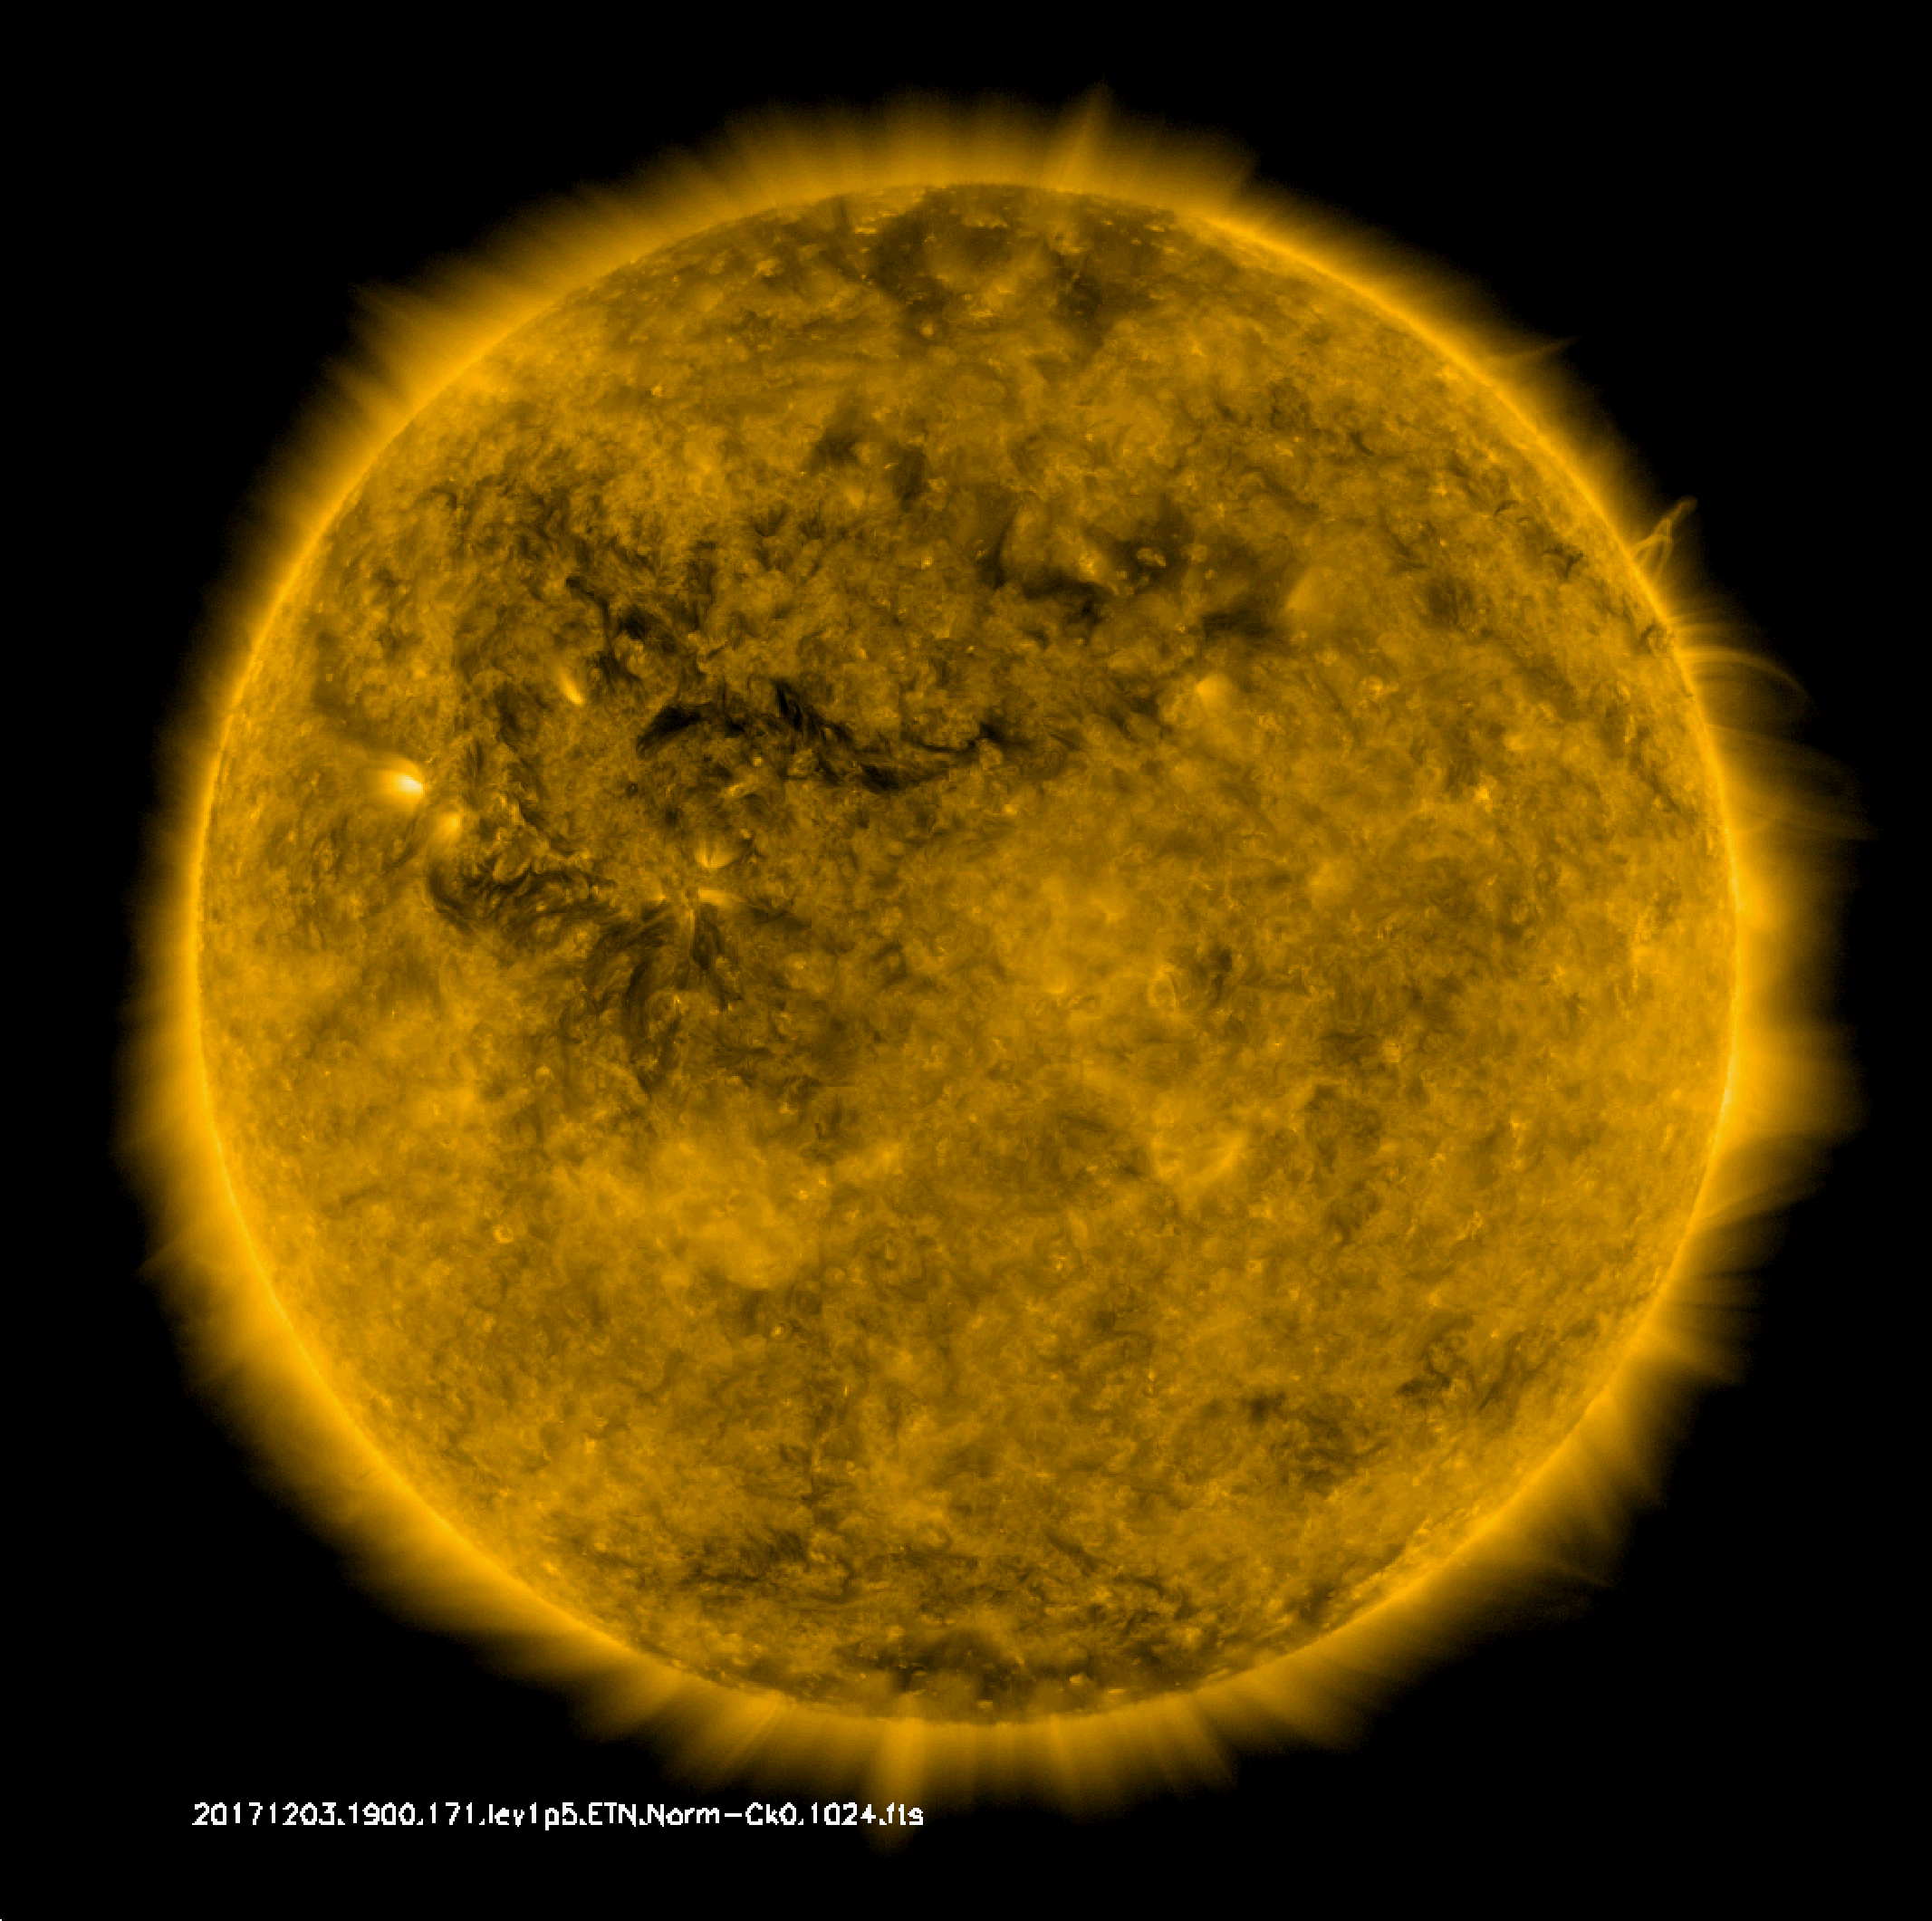
\includegraphics[width=0.15\textwidth]{figures/img_171.pdf}
  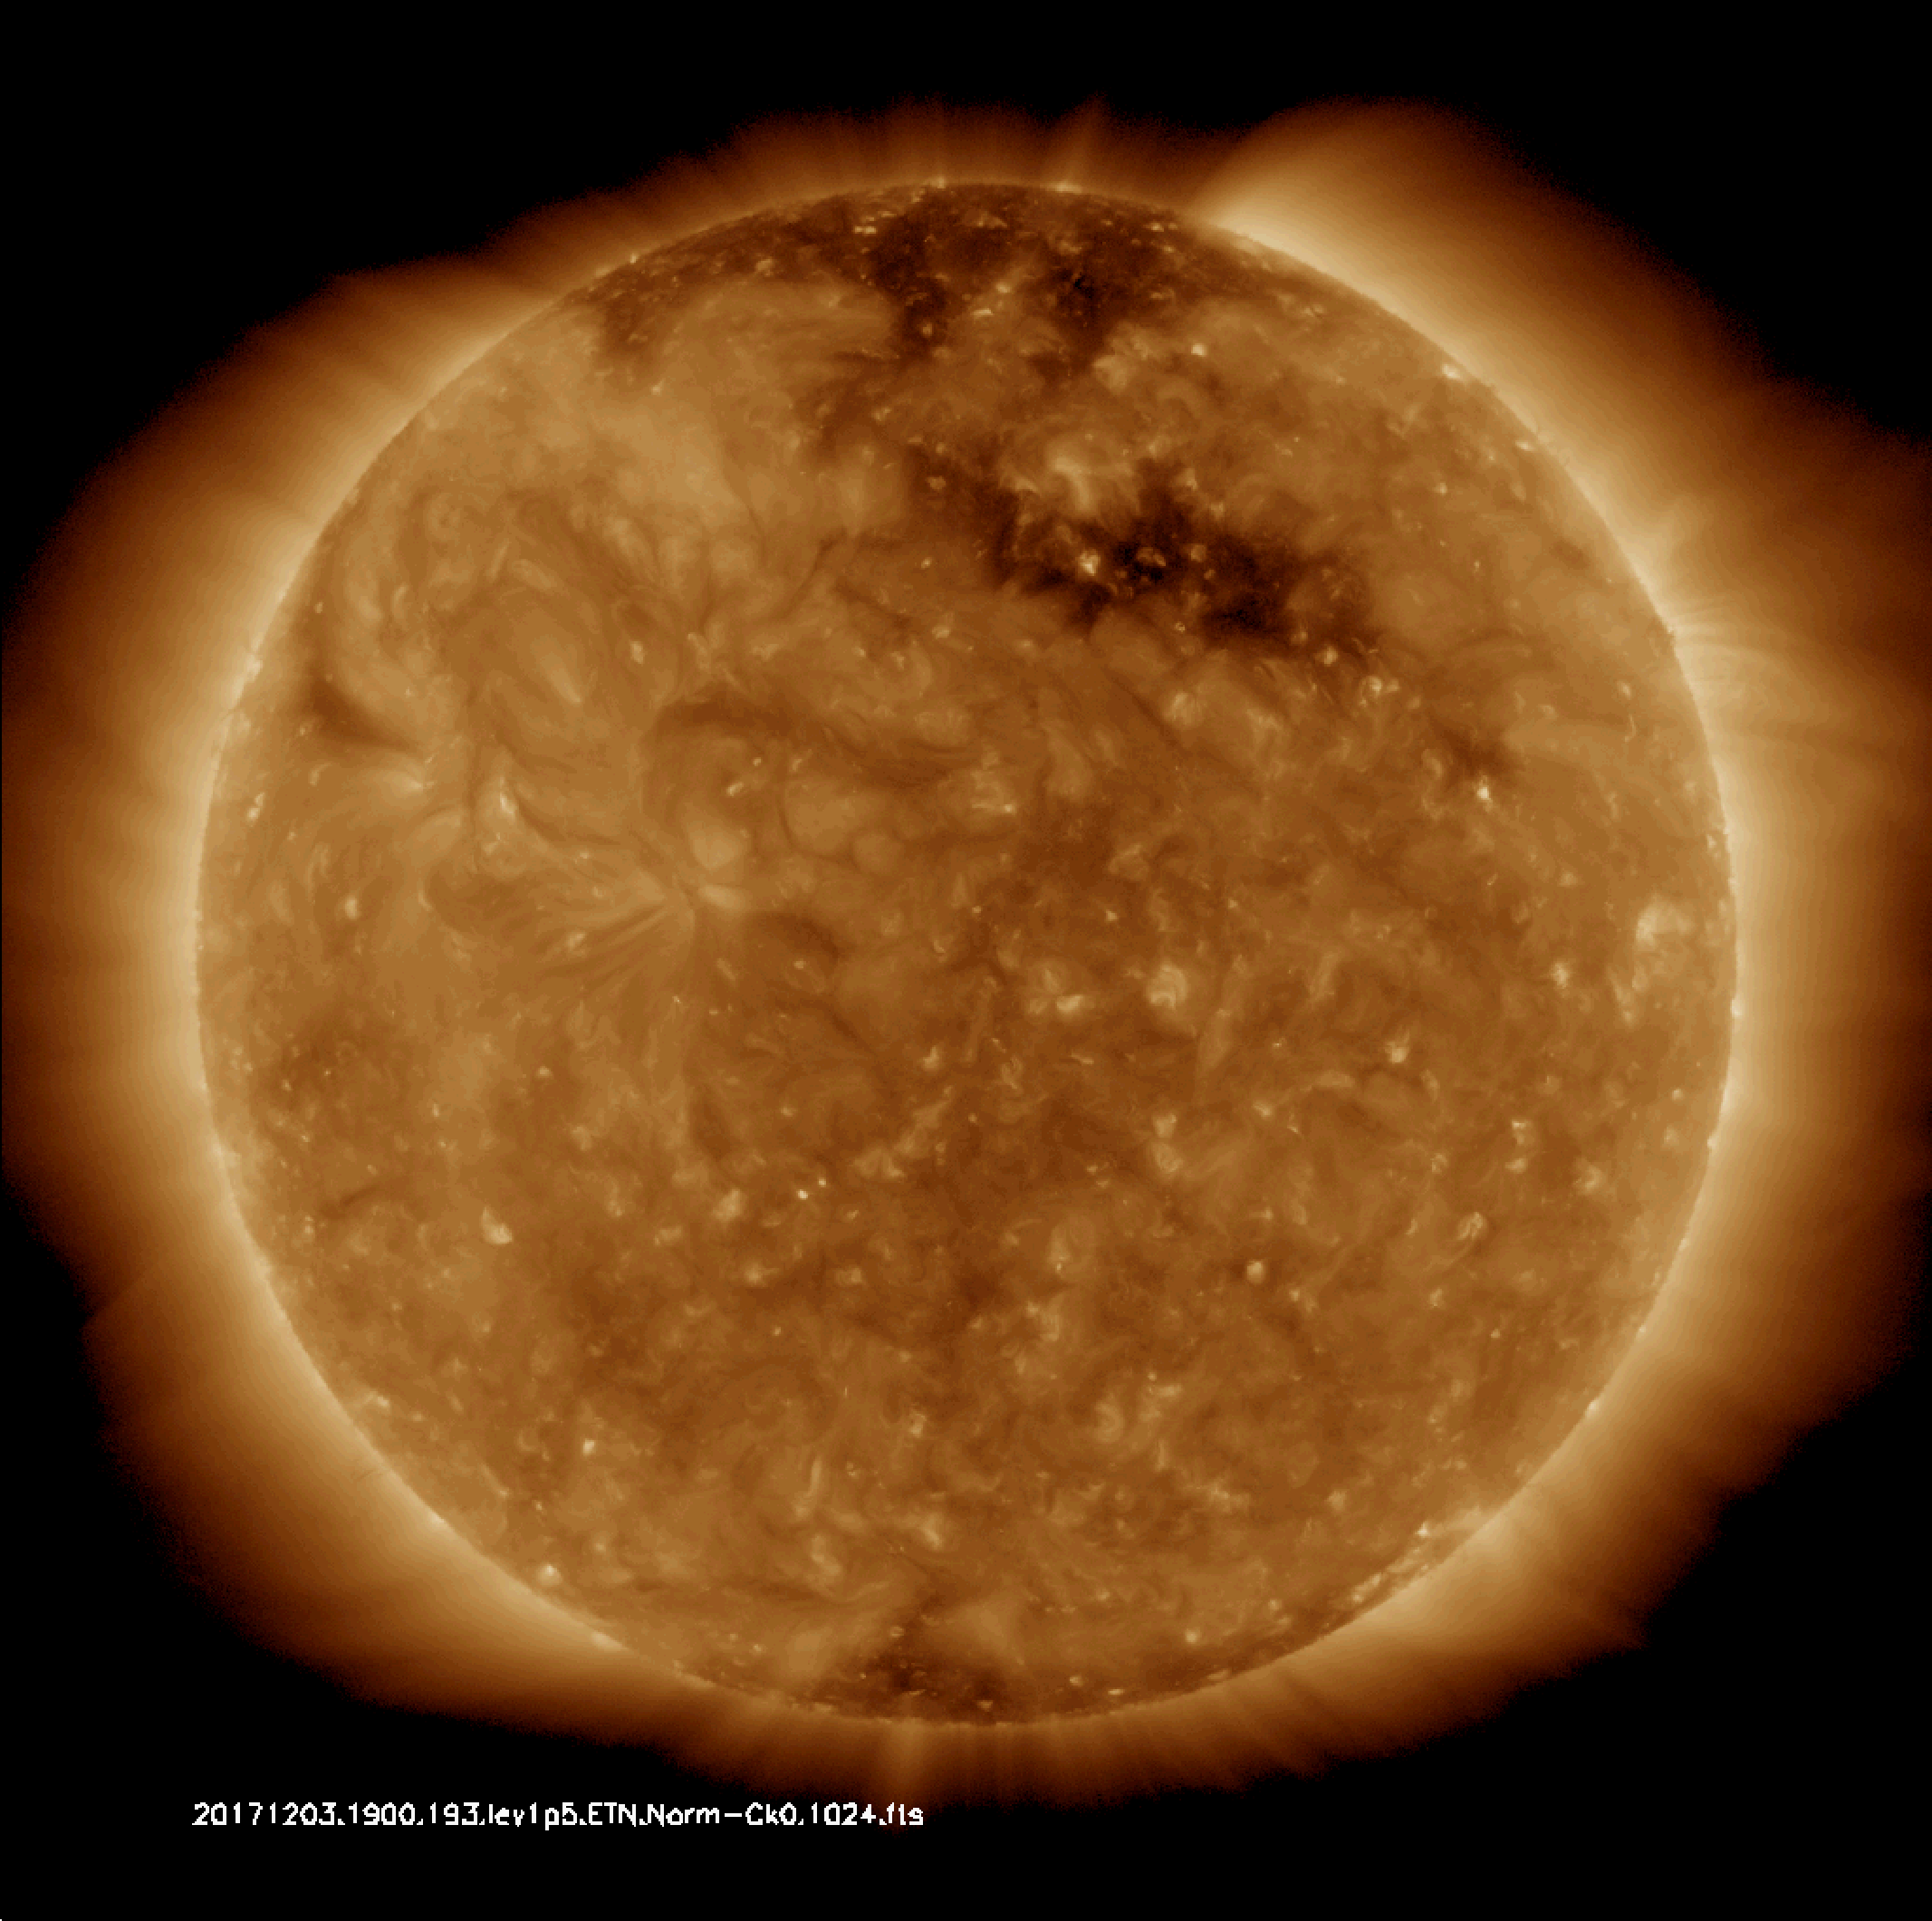
\includegraphics[width=0.15\textwidth]{figures/img_193.pdf}
  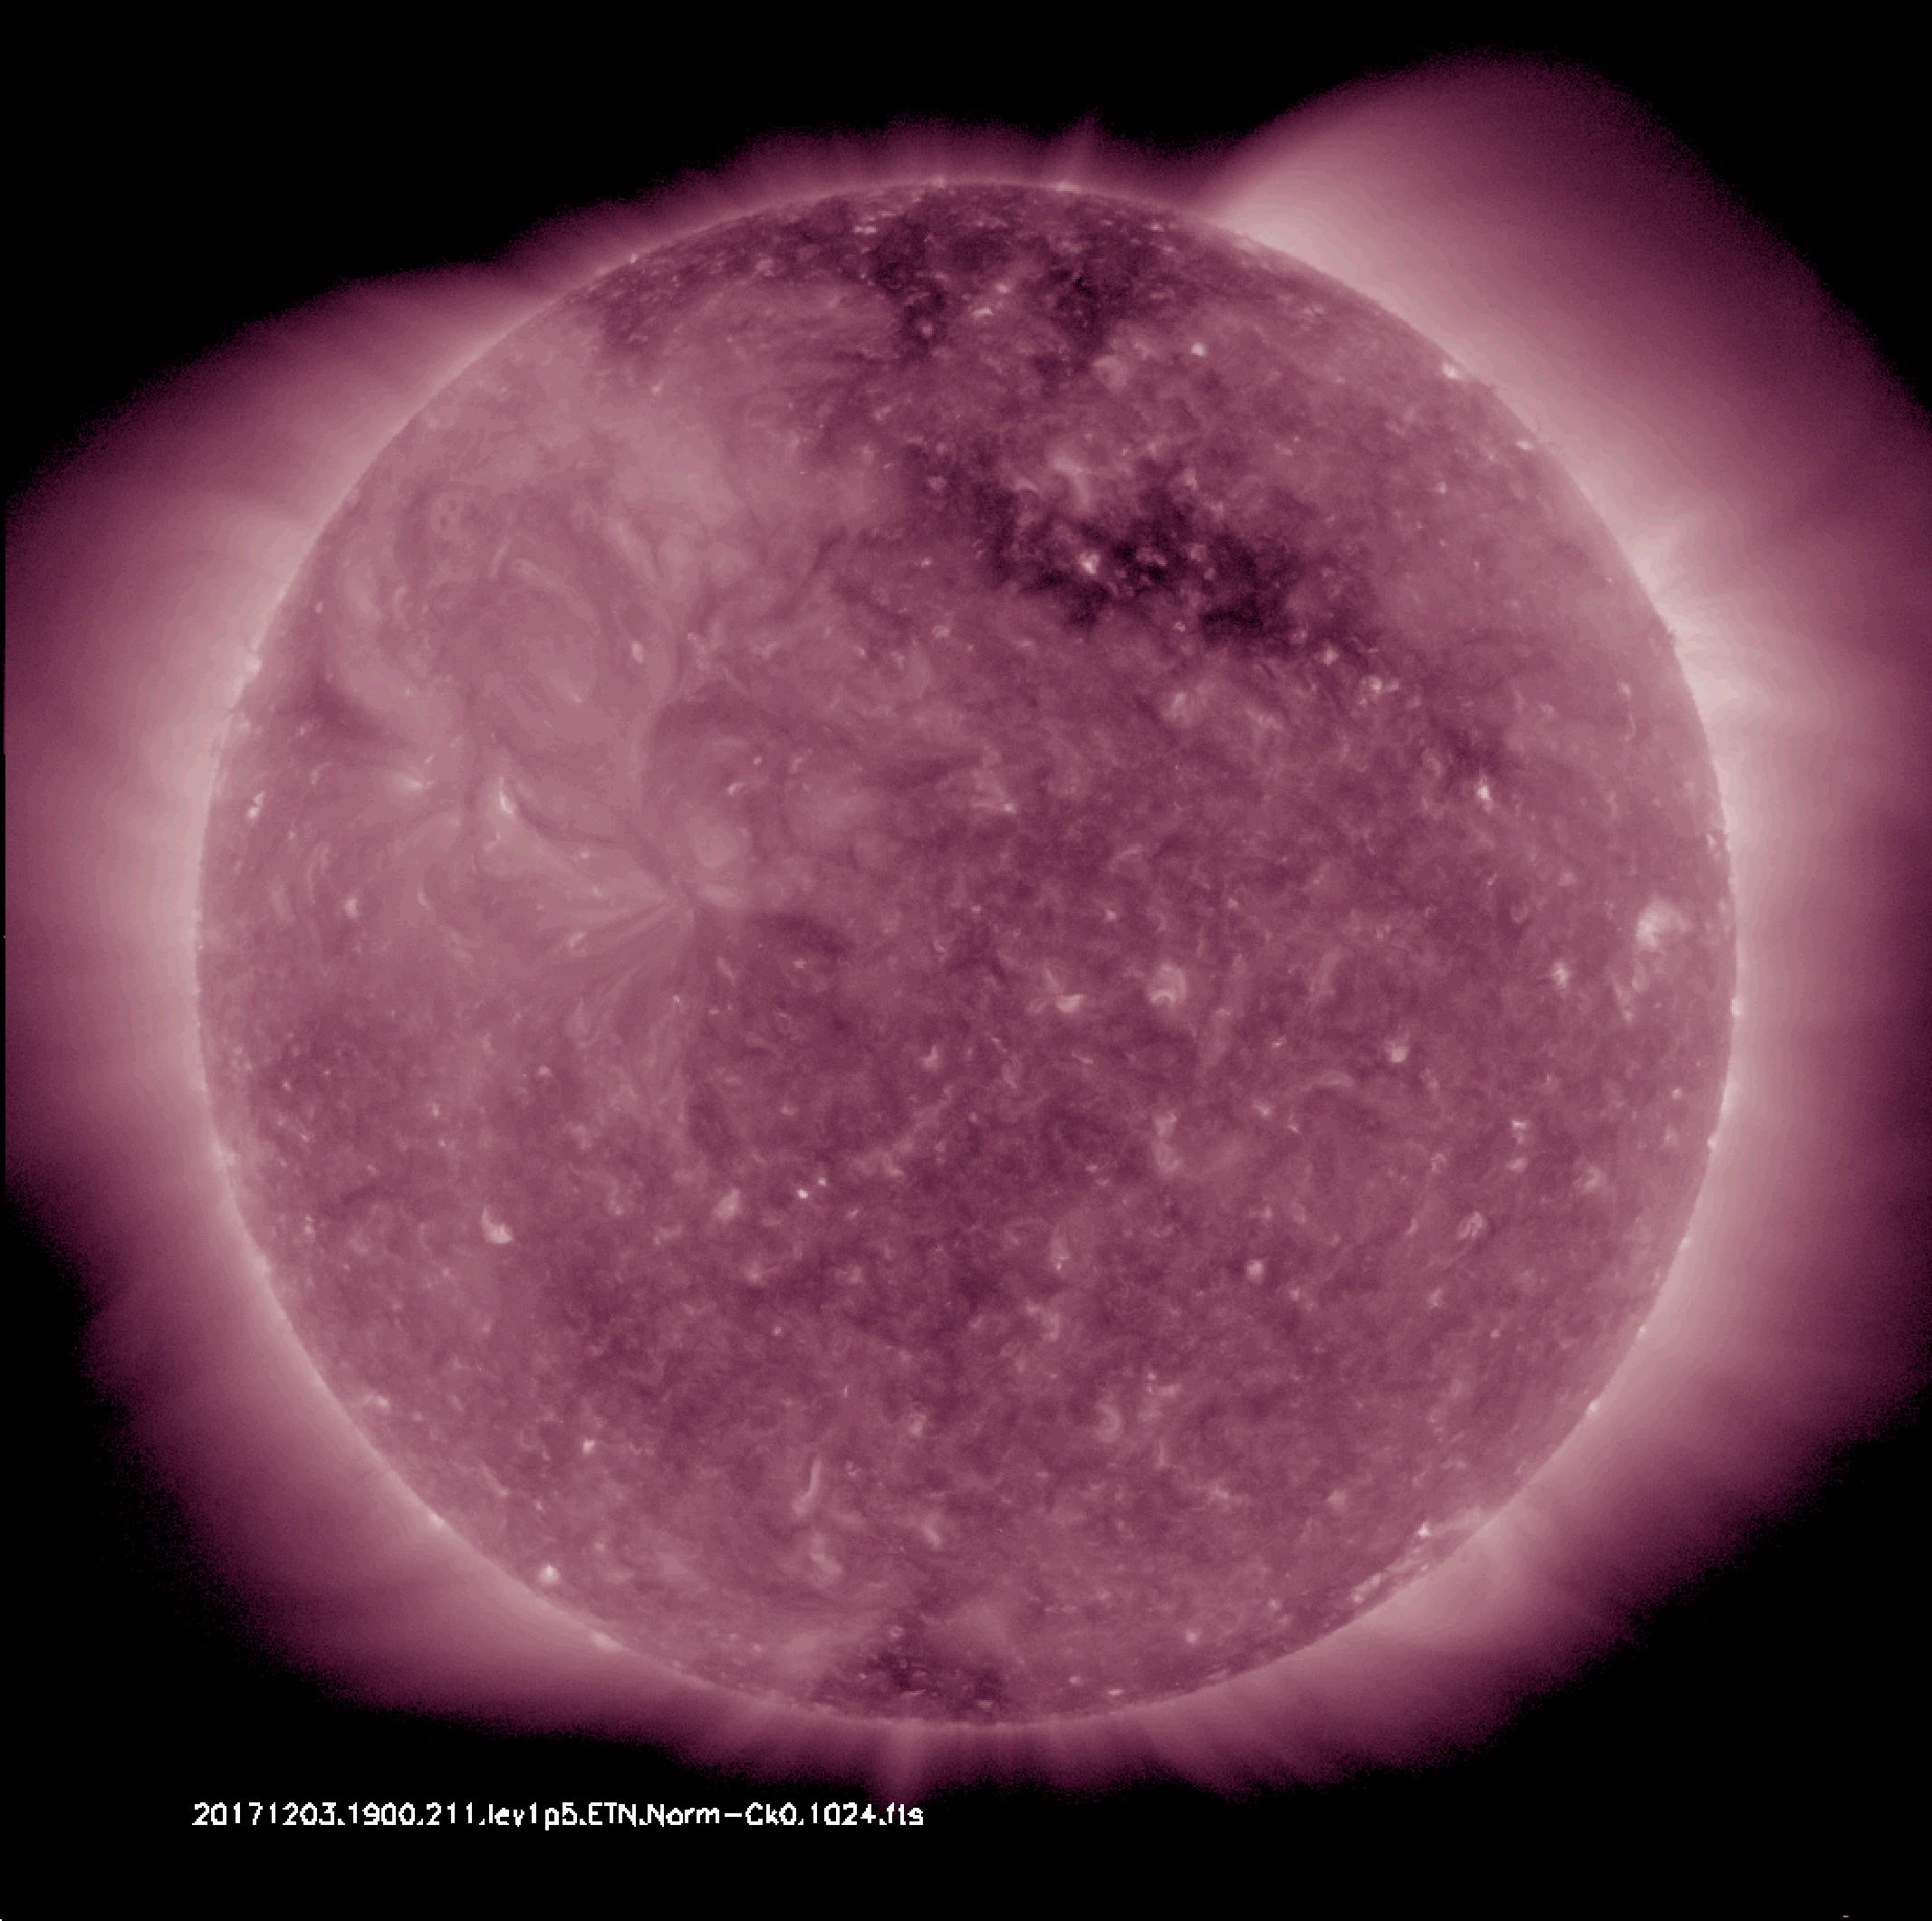
\includegraphics[width=0.15\textwidth]{figures/img_211.pdf}
  \caption{AIA/SDO.}
  \label{fig_00}
\end{figure}


\section{Results}

\begin{figure}
  \centering
  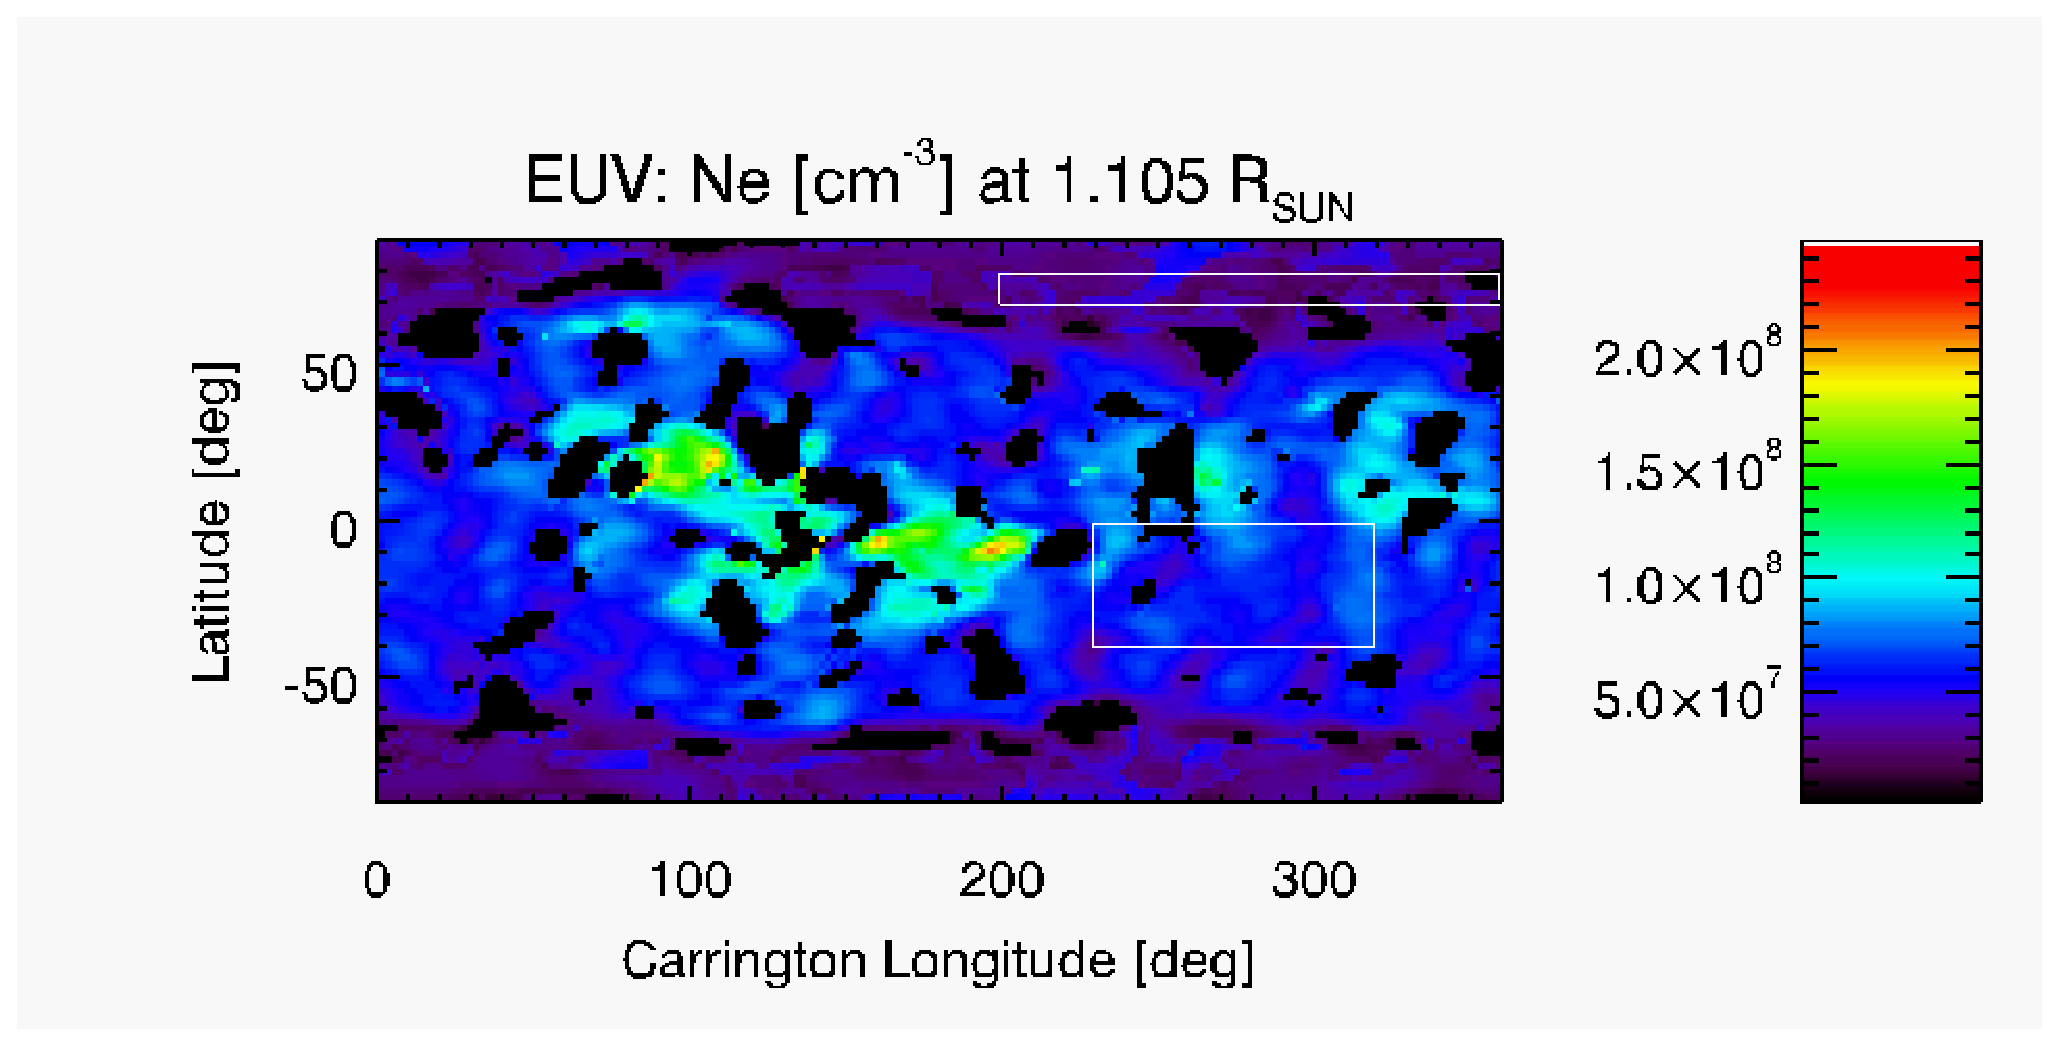
\includegraphics[width=0.4\textwidth]{figures/map_ne_aia.eps}\\
  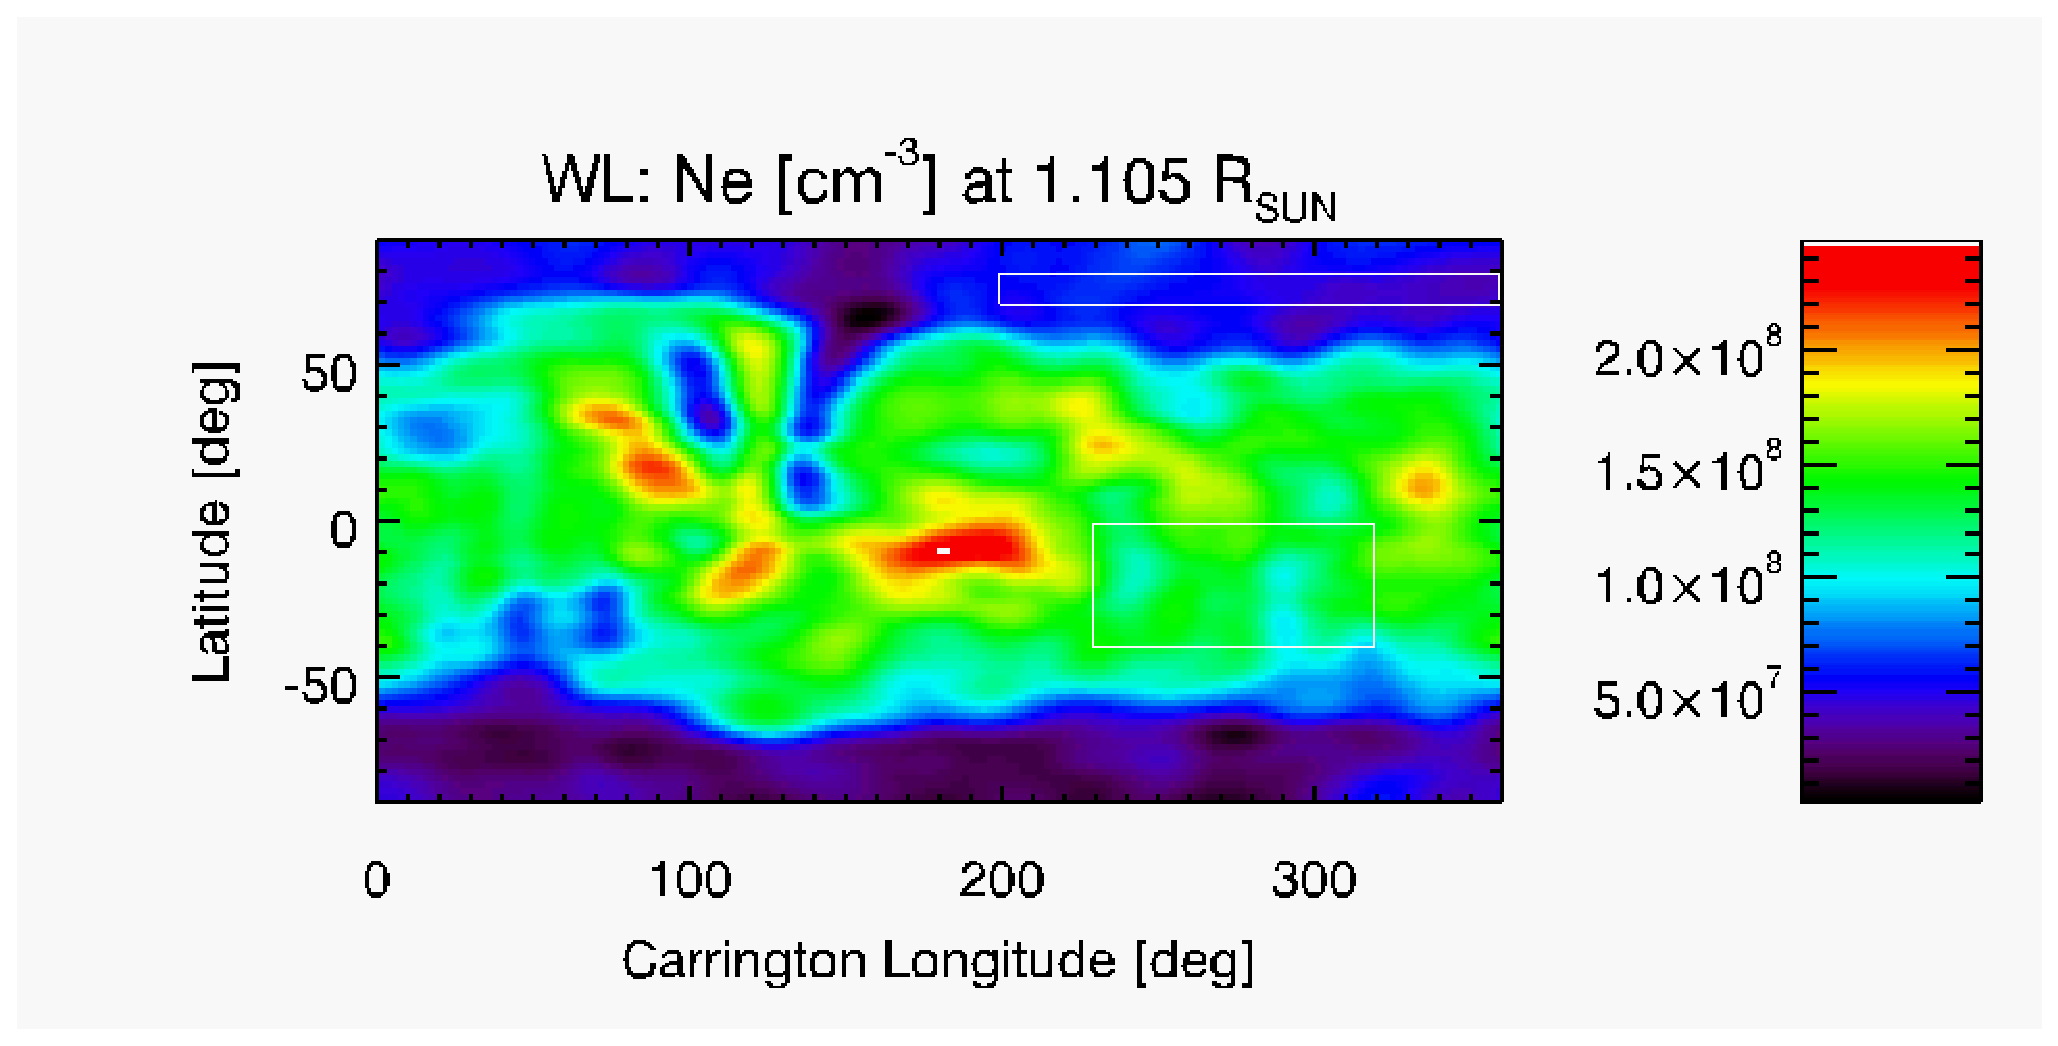
\includegraphics[width=0.4\textwidth]{figures/map_ne_kcor.eps}
  \caption{AIA/SDO.}
  \label{fig_maps}
\end{figure}

\begin{figure}
  \centering
  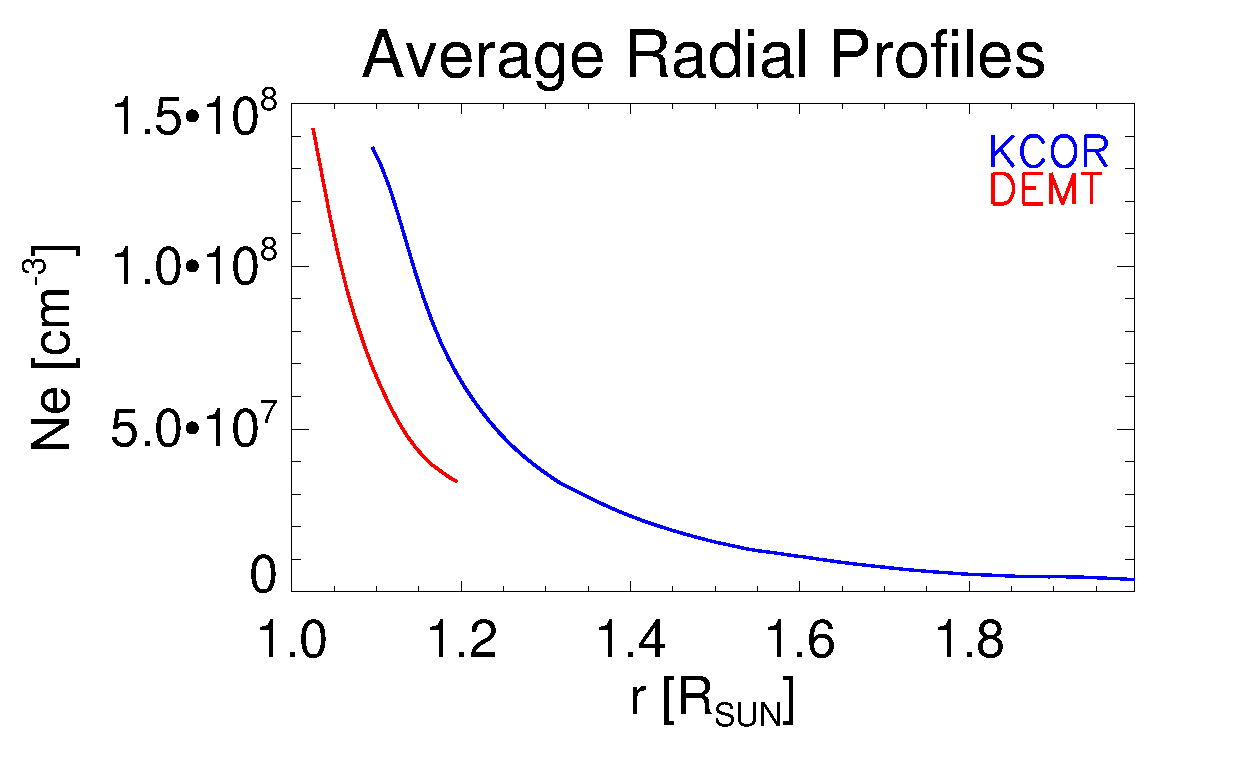
\includegraphics[width=0.3\textwidth]{figures/Average_Radial_Profiles_KCOR-Tom_vs_DEMT_CR2198_Hh_l45_kcor_subreg-Quiet-region1.eps}\\
  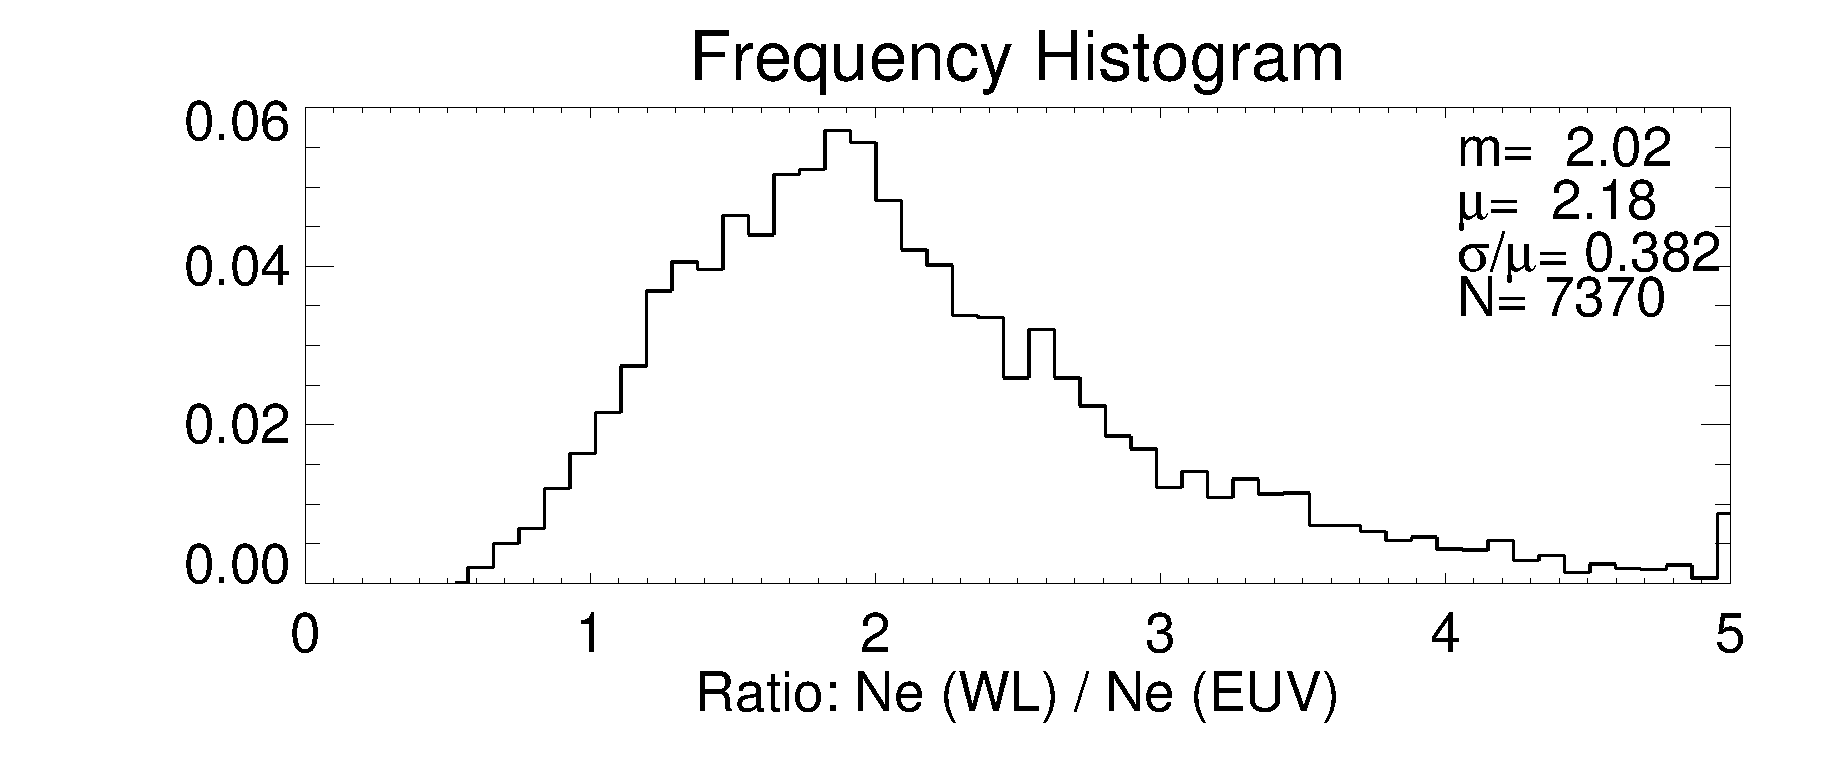
\includegraphics[width=0.4\textwidth]{figures/comparison_KCOR-Tom_vs_DEMT_CR2198_Hh_l45_kcor_subreg-Quiet-region1_range1105-1195_Rsun.eps}	
  \caption{AIA/SDO.}
  \label{fig_averages}
\end{figure}

\begin{figure}
  \centering
  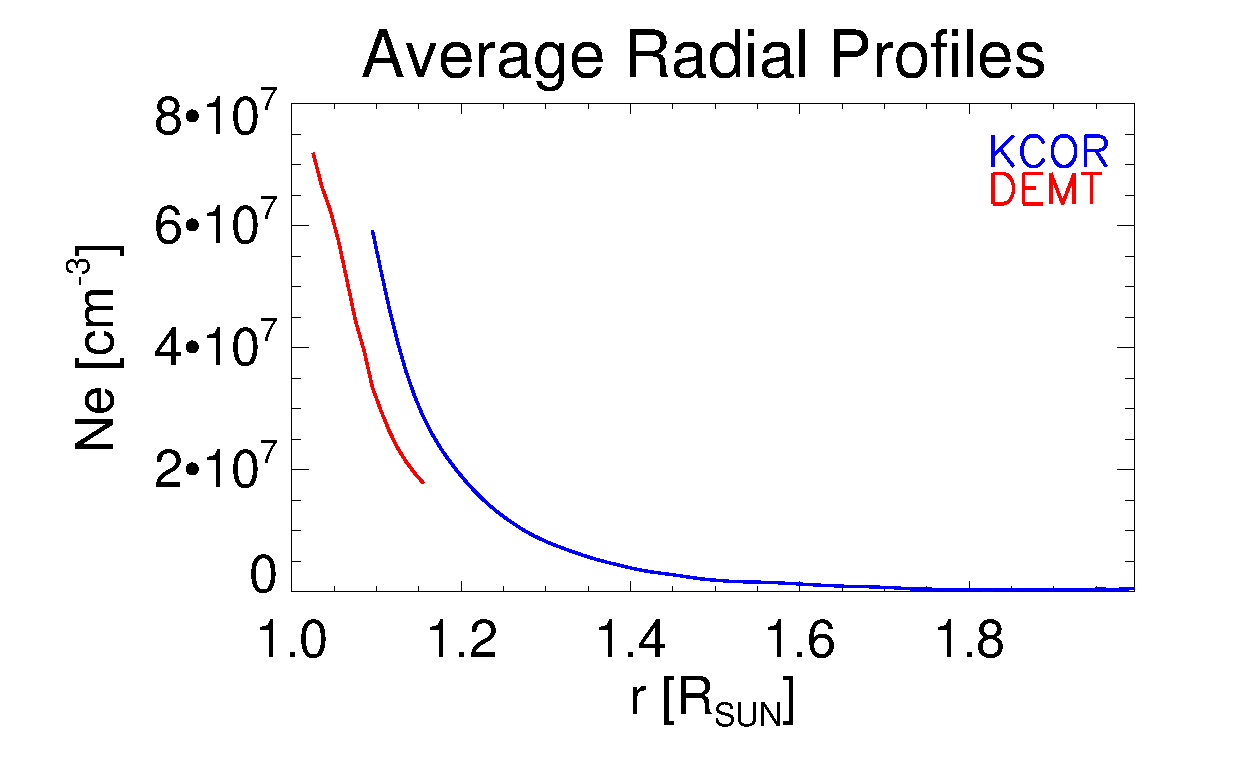
\includegraphics[width=0.3\textwidth]{figures/Average_Radial_Profiles_KCOR-Tom_vs_DEMT_CR2198_Hh_l45_kcor_subreg-Open-region_N.eps}\\
  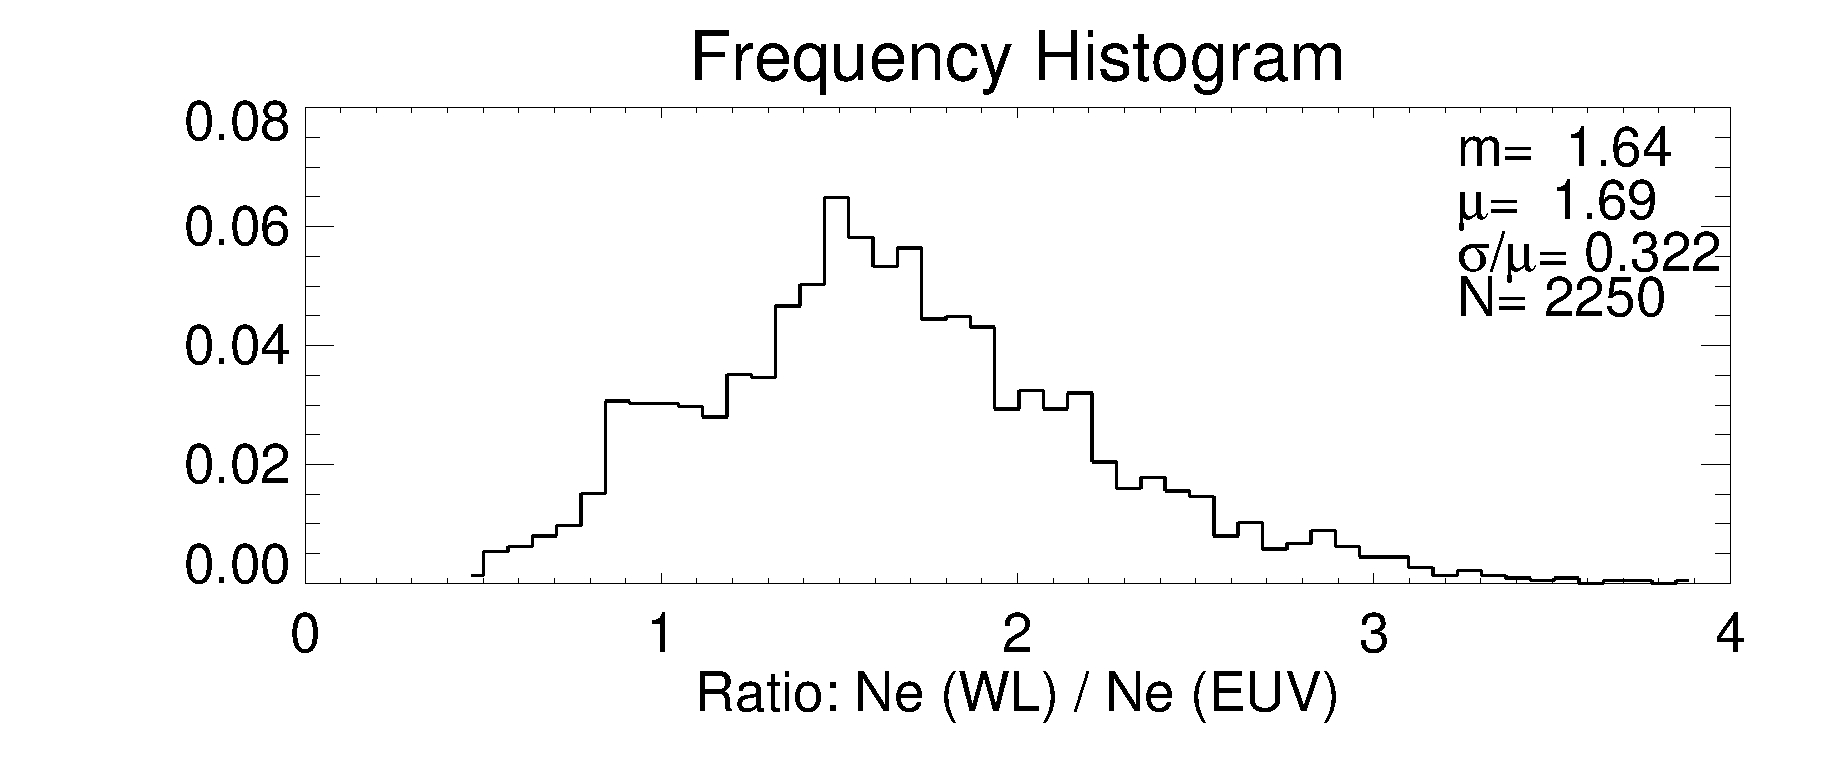
\includegraphics[width=0.4\textwidth]{figures/comparison_KCOR-Tom_vs_DEMT_CR2198_Hh_l45_kcor_subreg-Open-region_N_range1105-1155_Rsun.eps}	
  \caption{AIA/SDO.}
  \label{fig_comparisson}
\end{figure}


\section{Conclusions and future efforts}
\begin{itemize}
 \item  $\Eeuv \propto \AvgNE2 = f\,\AvgNe^2$, where \azul{filling factor} is defined as $f\equiv\AvgNE2 / \AvgNe^2$
\salto
\item  $\Ewl \propto \AvgNe$
\salto
\item  Then: $\AvgNe_{\rm{WL}} / \AvgNe_{\rm{EUV}} \propto \sqrt{f}$
\salto
\item  If differences in the results are solely attributed to filling factor:\\
  $f\sim 2$ in subpolar open region, and $f\sim 4$ in quiet sun closed region.
\salto
\item  Note that: $\SigmaNe^2 \equiv \rm{Var}N_e = \AvgNE2 - \AvgNe^2 = \AvgNe^2 \, (f-1)$
\salto
\item  So that: $\SigmaNe / \AvgNe = \sqrt{f-1}$.
\salto
\item  With this interpretation, where $f$ is larger (quiet sun closed region) the electron density probability distribution has larger variance.
\end{itemize}
%%%%%%%%%%%%%%%%%%%%%%%%%%%%%%%%%%%%%%%%%%%%%%%%%%%%%%%%%%%%%%%%%%%%%%%%%%%%%%
%                                                                            %
%  Por favor no modifique las líneas de la bibliografía, salvo el nombre     %
%  el archivo de Bibtex con la lista de citas (sin la extensión .BIB)        %
%                                                                            %
%  Please do not modify the following lines, except the name of the Bibtex   %
%  file (whithout the .BIB extension)                                        %
%                                                                            %
%%%%%%%%%%%%%%%%%%%%%%%%%%%%%%%%%%%%%%%%%%%%%%%%%%%%%%%%%%%%%%%%%%%%%%%%%%%%%% 

\bibliographystyle{baaa}
\small
\bibliography{BAAA60_Diego_Lloveras}
 
\end{document}
